\chapter{Стабилизация с реальным дифференцирующим звеном}
\label{ch:chap2}


Заменим блок аппроксимации производной \textit{derivative} на передаточную функцию вида:
$$
W_{diff}(s) = \frac{s}{Ts+1}
$$
\begin{figure}[ht]
  \centering
  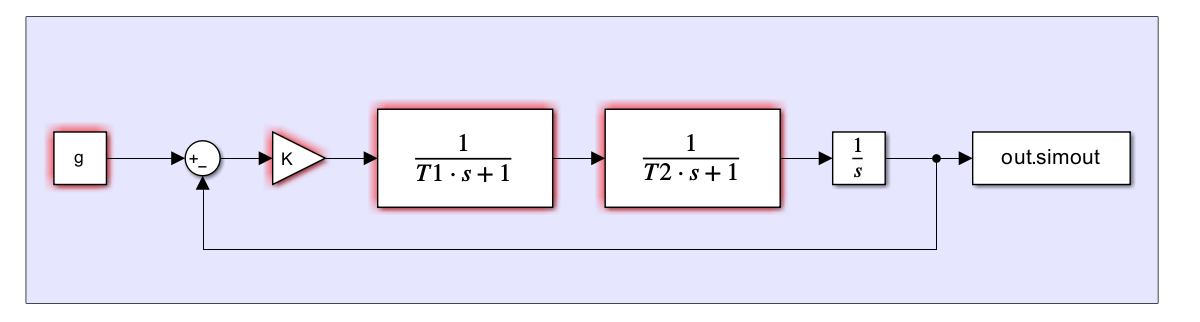
\includegraphics[width=0.8\textwidth]{scheme_system2.png}
\caption{Структурная схема - новая передаточная функция}
\end{figure}

Определим критические значения параметра $T$, для этого воспользуемся преобразованием Лапласа, а также ранее определённые константы регулятора:
$$
\begin{aligned}
  a_2s^2Y(s) + a_1sY(s)+a_0Y(s) + 0 = k_0Y(s) + k_1Y\frac{s}{Ts+1} 
\end{aligned}
$$
где $+0$ - обнулённые начальные условия, посколько сейчас нас волнует вопрос устойчости -, а это только знаменатель от $Y(s)$
$$
\begin{aligned}
  s^2Y(s) -2sY(s)-3Y(s) + 0 = -6Y(s) -4Y\frac{s}{Ts+1}  \\
  s^2Y(s) -2sY(s)+3Y(s) = -4Y\frac{s}{Ts+1} \bigg|\cdot Ts+1 \\
  \dots \\
  s^3Y(s) + s^2Y(s)(\frac{1-2T}{T}) +sY(s)(\frac{3T+2}{T}) + \frac{3}{T} = 0
\end{aligned}
$$
Воспользуемся критерием Гурвица для системы третьего порядка:
$$
\begin{cases}
  T>0 \\
  3T+2 > 0 \\
  1-2T > 0 \\
  \frac{(3T+2)(1-2T)}{T^2} > \frac{3}{T}
\end{cases}
$$
$$
\begin{cases}
  T \in (0, \frac{1}{2}) \\
  (3T+2)(1-2T) > 3T
\end{cases}
$$
В итоге получим следующий интервал: $T\in(0;\frac{1}{3})$.

Проведём несколько экспериментов при разных $T$, сведём их в один график для сопоставления:
$$
T_1 = 1/4, T_2 = 1/12, T_3 = 1/24, T_4 = 1/48
$$
\begin{figure}[ht]
  \centering
  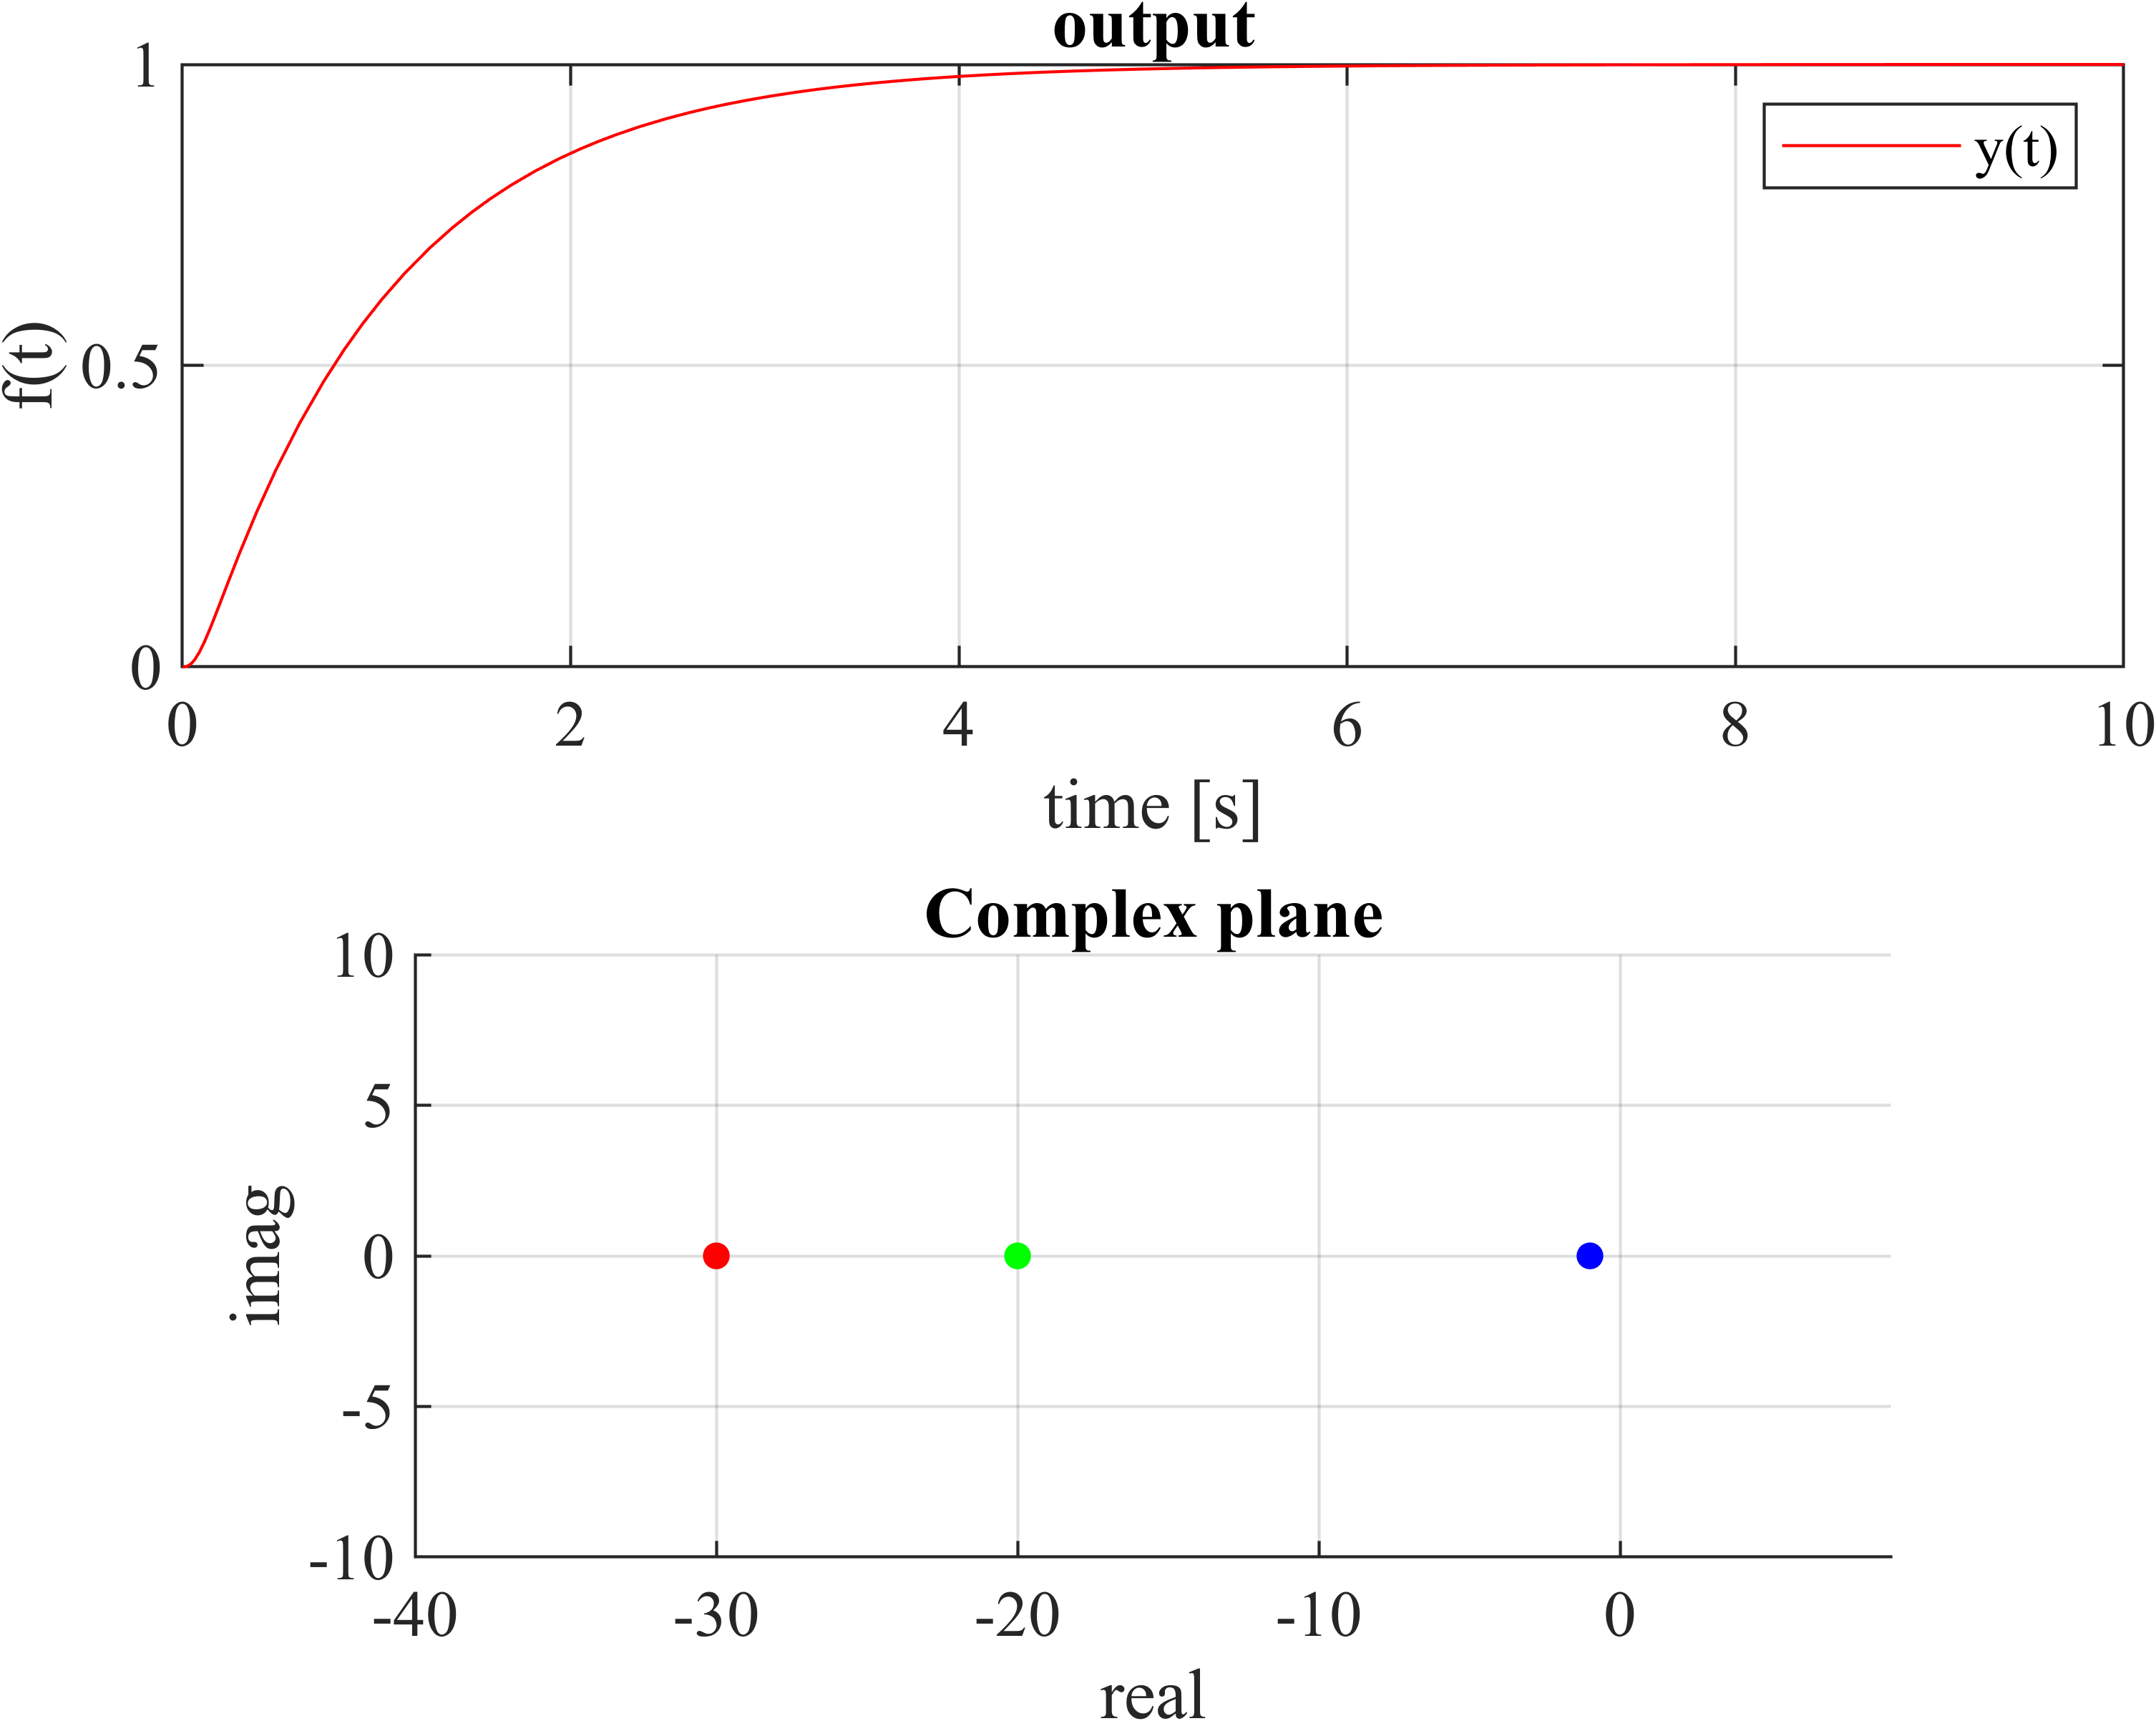
\includegraphics[width=1.0\textwidth]{output_task2_exp5.png}
\caption{Симуляция - устойчивость при $T=1/4$}
\end{figure}

\newpage
\begin{figure}[ht]
  \centering
  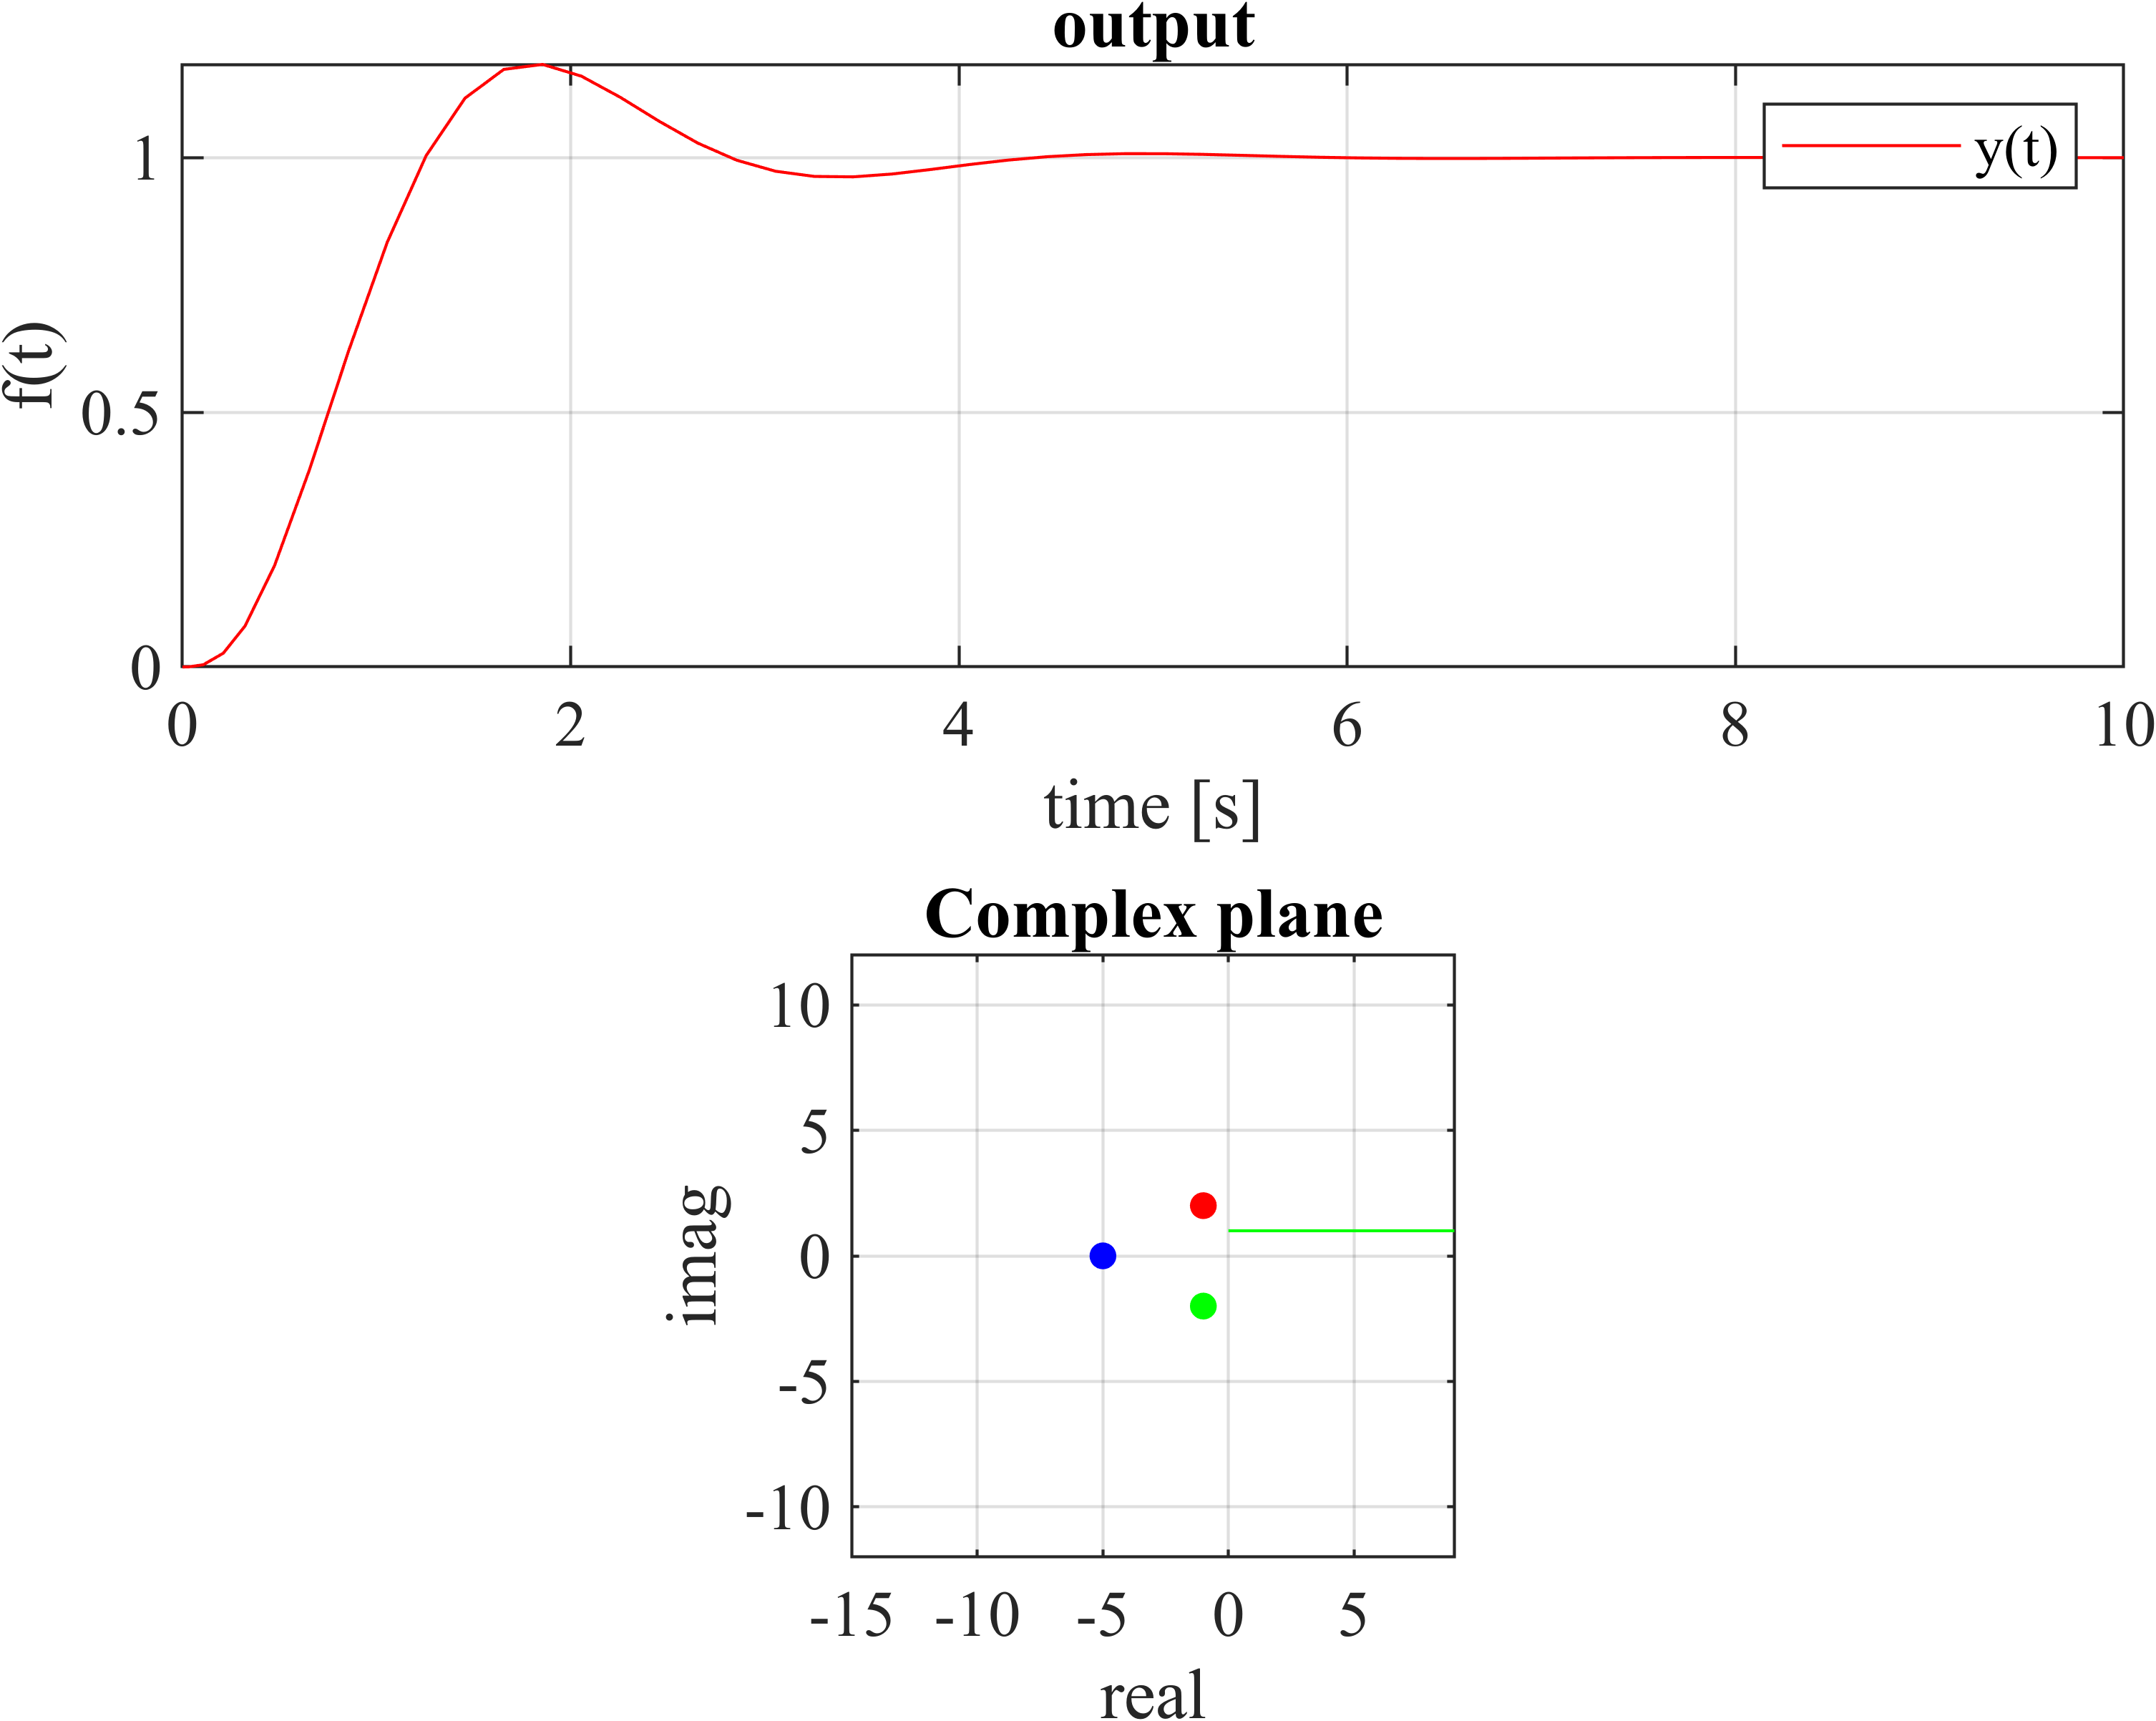
\includegraphics[width=0.8\textwidth]{output_task2_exp6.png}
\caption{Симуляция - сравнение задание 1/2}
\end{figure}

\textbf{Выводы:} Как можно заметить, при уменьшении параметра $T$ к нулю, у нас улучшается регулирование - уменьшается перерегулирование (убираем колебания системы) и время переходного процесса.

Разница между аппроксимацией производной с помощью специального блока из \textit{simulink} или с помощью передаточной функции довольна заметна на сранвительном графике - но при хорошо подобранном $T$(достаточно маленьком) наша аппроксимация с помощью блока передаточной функции примерно также быстро сходится 
в ноль, также как и блоковая аппроксимация, хотя она все равно быстрее. Думаю, что передаточная функция в качестве аппроксимации менее вычислительно требовательная, нежели блок симулинка.

\endinput